\chapter{Background}\label{chap:background}
% \begin{algorithm}[p]
\caption{Stochastic Gradient Descent: Neural Network}
\label{alg:backpropnn}
\begin{algorithmic}
    % \ttfamily
    \State Create a mini batch of $m$ samples $\vec{x}_0 \ldots \vec{x}_{m-1}$
    \ForEach{sample $\vec{x}$}
        \State $\vec{a}^{\vec{x},0} \gets \vec{x}$  \alignedComment{Set input activation}
        \ForEach{Layer $l \in \{1\ldots L-1\}$}  \alignedComment{Forward pass }
            \State $\vec{z}^{\vec{x},l} \gets \mathbf{W}^l \vec{a}^{\vec{x},l-1}+\vec{b}^l$
            \State $\vec{a}^{\vec{x},l} \gets \varphi(\vec{z}^{\vec{x},l})$
        \EndFor
        \State $\bm{\delta}^{\vec{x},L} \gets \nabla_{\vec{a}} C_\vec{x} \odot \varphi'(\vec{z}^{\vec{x},L})$ \alignedComment{Compute error}
        \ForEach{Layer $l \in L-1, L-2 \ldots 2$}  \alignedComment{Backpropagate error}
            \State $\bm{\delta}^{\vec{x},l} \gets ((\mathbf{W}^{l+1})^T \bm{\delta}^{\vec{x},l+1})\odot \varphi'(\vec{z}^{\vec{x},l})$
        \EndFor
    \EndFor
    \ForEach{$l \in L, L-1 \ldots 2$} \Comment  \alignedComment{Gradient descent}
        \State $ \mathbf{W}^l \gets \mathbf{W}^l-\frac{\eta}{m} \sum_\vec{x} \bm{\delta}^{\vec{x},l} (\vec{a}^{\vec{x},l-1})^T$
        \State $\vec{b}^l \gets \vec{b}^l-\frac{\eta}{m}\sum_\vec{x} \bm{\delta}^{\vec{x},l}$  
    \EndFor
\end{algorithmic}
\end{algorithm}
% 
%
% \begin{figure}[t]
%     \begin{center}
%     \begin{tikzpicture}
%         \node (a) at (0,0) {a};
%         \node (b) at (2, 0) {b};
%         \draw[->] (a) -- (b);
%
%
%     \end{tikzpicture}
%     \end{center}
%     \caption[Tikz Example]{Use tikz to draw nice graphs!}
%     \label{fig:Tikz}
% \end{figure}


\section{Chromosome Conformation Capture and Hi-C}\label{sec:c3}\label{sec:hic}

\begin{figure}[t]
\begin{centering}
%    \subfloat[Diagram summarising the Hi-C experimental protocol. The red and blue rectangles represent cross-linked restriction fragments while the yellow marker shows the position of biotin incorporation.]
%    \subfloat[Generation of the Hi-C ligation junction sequence by successive digestion (with HindIII in this example), fill in and blunt-ended ligation steps. The modified restriction site sequence is not found in the original genomic sequence.]
    {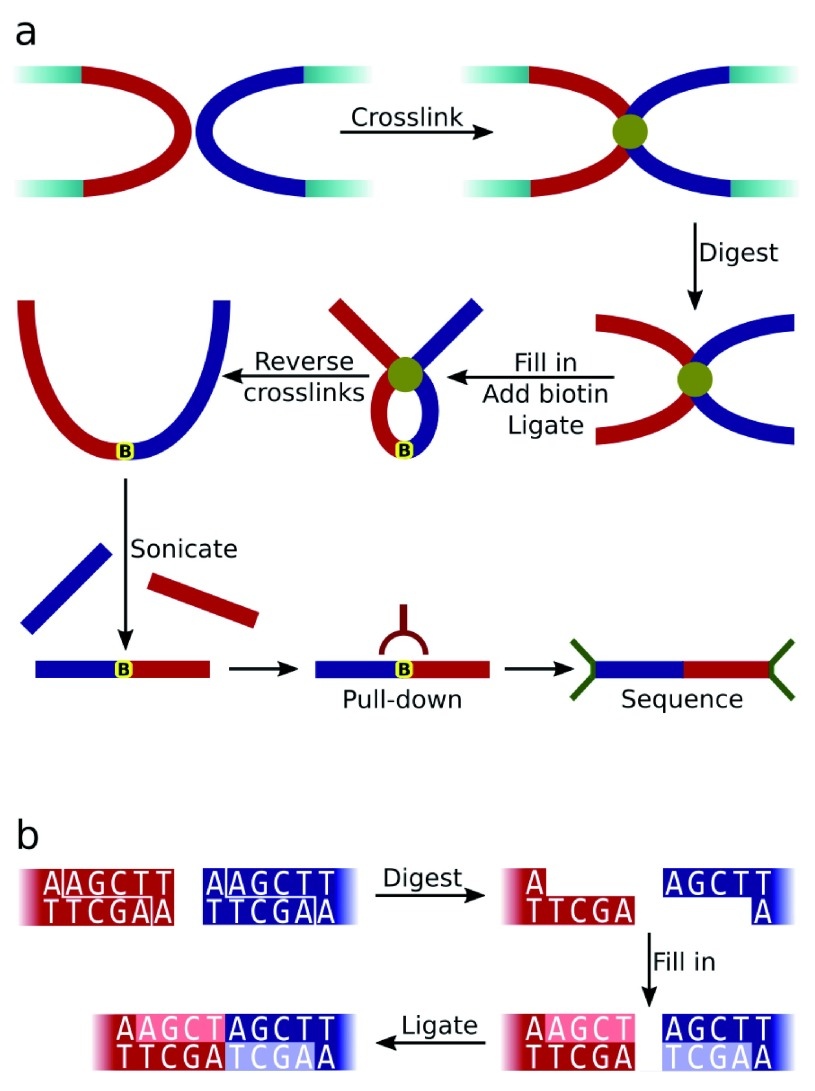
\includegraphics[scale=4]{figures/background/f1000research-4-7903-g0000.jpg}}
    \caption[Summarised Hi-C protocol]
    {\textbf{a)} Diagram summarising the Hi-C experimental protocol. The red and blue rectangles represent cross-linked restriction fragments while the yellow marker shows the position of biotin incorporation. \textbf{b)} Generation of the Hi-C ligation junction sequence by successive digestion (with HindIII in this example), fill in and blunt-ended ligation steps. The modified restriction site sequence is not found in the original genomic sequence. \\ \\ Image and description taken from \cite{wingett2015hicup}.}
    \label{fig:HiC}
    \todo{rewrite the description in my own words}

    \todo{remove the b section}
\end{centering}
\end{figure}



    % {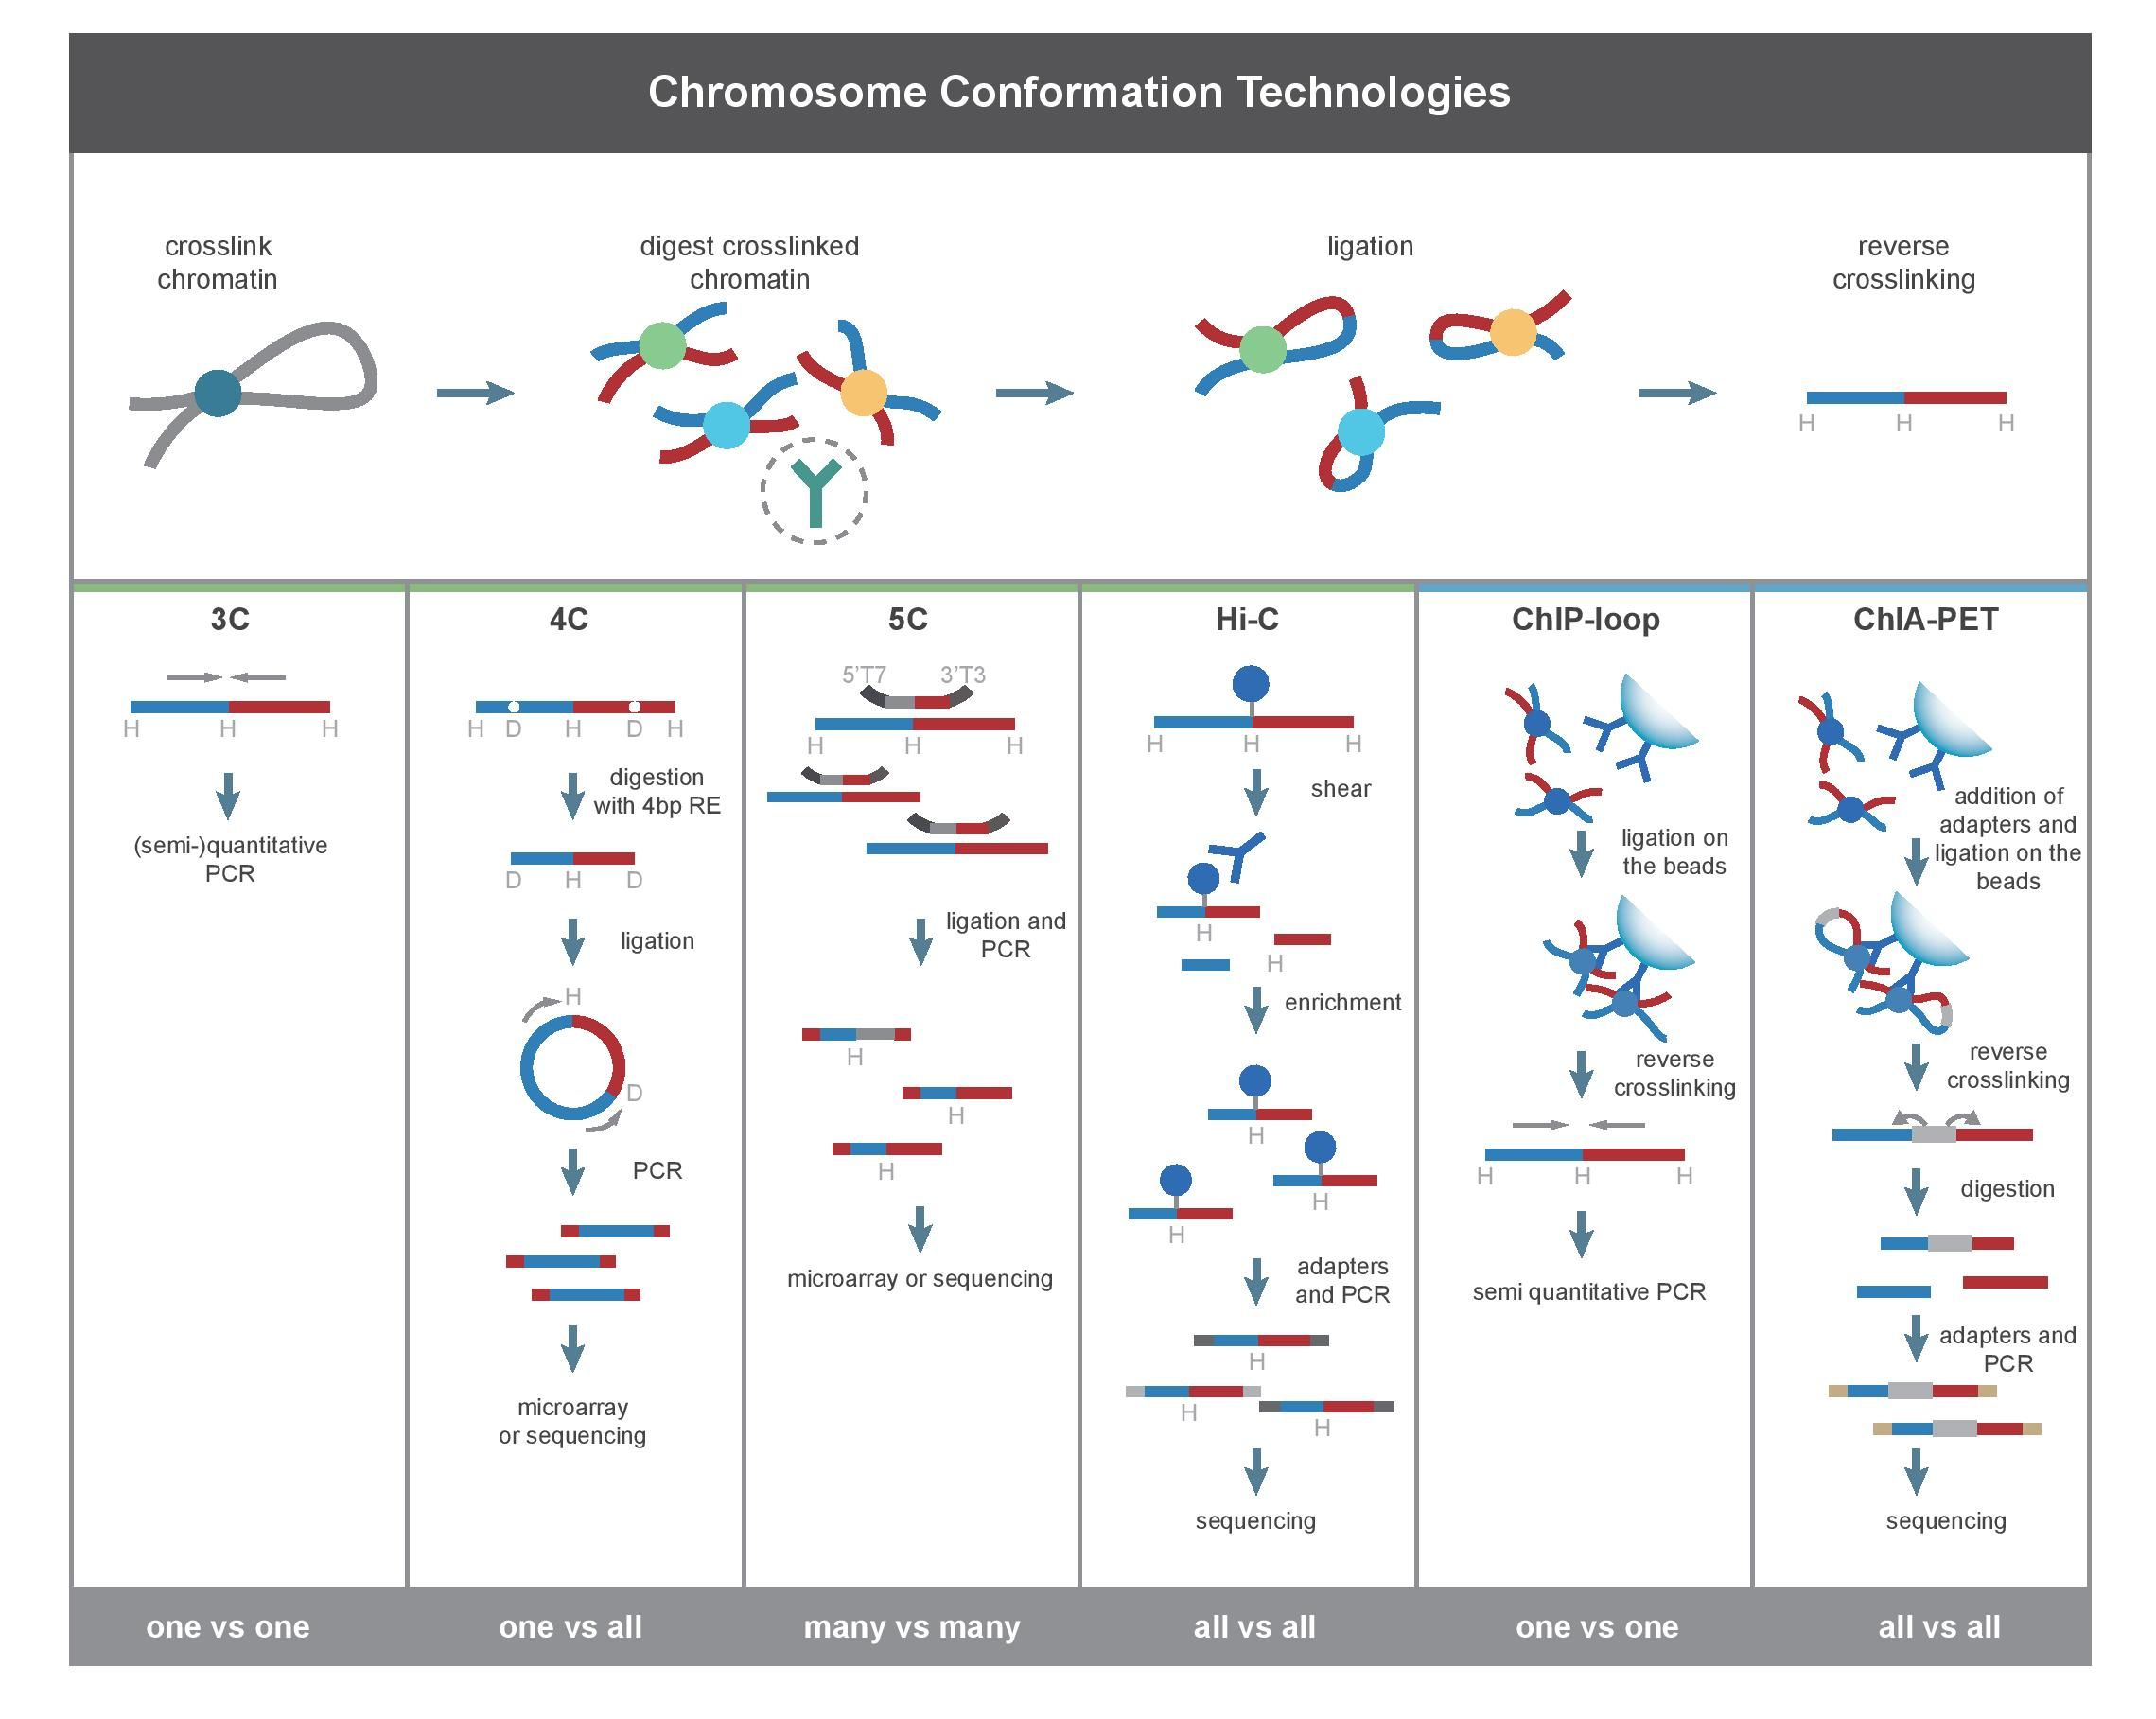
\includegraphics[scale=0.8]{figures/background/Chromosome_conformation_techniques.jpg}}
    % \caption[Comparison among 3C and its derived methods]{\textbf{Comparison among 3C and its derived methods} Source: https://en.wikipedia.org/wiki/File:Chromosome\_conformation\_techniques.jpg}


\subsection{Overview}


Chromatin usually describes different levels of how DNA organizes itself. The
well-known double-helix is only the lowest of several structural layers.

Looking at it from the outside (highest structural layer), DNA looks similar to
a big ball of wool. With the help of Hi-C (or other methods) we can visualize
the spatial proximity.

% Gene markers tend to also have effect on their spatial neighbourhood, not only on the neighbourhood going up and down the strand of DNA.



Chromosome Conformation Technologies describe several similar methods to
compare genomic loci. They all start by:

\begin{itemize}
    \item creating chromatin cross-links (\secref{sec:crosslinking}),
    \item digesting the cross-linked chromatin (\secref{sec:digestion}),
    \item ligating the ends and marking with Biotin (\secref{sec:ligation}) and
    \item reversing the cross-link (\secref{sec:revcrosslink})
\end{itemize}

to get a sequence with two parts, those parts have been spatially close
to each other and were marked with Biotin during ligation.

Other Chromosome Conformation Technologies proceed differently, Hi-C, our
focus, continues with the following steps:

\begin{itemize}
    \item shortening the cross-links by sonication (\secref{sec:sonication}),
    \item filtering leaving only those with biotin (\secref{sec:pulldown}) and
    \item sequencing (\secref{sec:sequencing}).
\end{itemize}

The full process can be seen in \figref{fig:HiC}.

\subsection{Cross-linking DNA}\label{sec:crosslinking}

The first step is to cross-link DNA strands that are close to each other
spatially (see \figref{fig:HiC} for reference). This is done by adding
formaldehyde, which bonds (links) sufficiently close strands together.

A chromatin cross-link is two entirely different parts of the genome held
together by a chemical bond with formaldehyde. This process cannot be
specifically controlled, so only `regions near each other' are connected, not
necessarily two `known to be close' regions.

\subsection{Digestion}\label{sec:digestion}

The next step is cutting the ball of wool apart in intervals. For this,
restriction-enzymes are used (specifically restriction endonuclease). Commonly
used enzymes for this are EcoR1 or HindIII, cutting the genome every 4000 base-pairs
\draft{info taken from Wikipedia, add some other source}.

This will result in a lot of cross-linked fragments, as well as not-cross-linked ones.

\subsection{Ligation}\label{sec:ligation}

After reducing the concentration of fragments, DNA ligase is added, to ligate
(weld together) dangling fragment ends. The reduction in concentration is done
since mostly fragments close together are ligated, and we intend to ligate
fragments held together by formaldehyde. Also, Biotin is added to mark the
points of ligation. This will let us filter out a lot of fragments that have
not been ligated later on.


\subsection{Reverse Cross-links}\label{sec:revcrosslink}

% Source: http://www.protocol-online.org/biology-forums/posts/10475.html
Adding a high concentration of salt for some time will reverse the
cross-linking through formaldehyde, leaving us with our two originally
spatially close fragments ligated and with a biotin-marker.

Our fragments, however, are too long to sequence them effectively (remember
that we have now ligated fragments of around 8000 base-pairs, most sequencing
methods can only deal with sequence lengths of a few hundred base-pairs).

\subsection{Sonication}\label{sec:sonication}

The next step is to put them under influence of ultrasonic waves, breaking them
apart in much shorter fragments (due to long sequences not being able to absorb
frequent shocks well), short enough to actually enable sequencing.

\subsection{Filtering and Removal of Biotin}\label{sec:pulldown}

Here we `pull-down' fragments marked with biotin, filtering all the fragments
and leaving only those having been ligated earlier (see \secref{sec:ligation}).
Subsequently we remove the marker, since it would get in the way of sequencing.

\subsection{Sequencing}\label{sec:sequencing}

Sequencing, short for DNA sequencing, describes processes of measuring a DNA
sequence. There are several techniques for doing this, most use PCR (Polymerase
Chain Reaction) before or while sequencing, which duplicates the fragments
several times, to sequence them more accurately.

% - putting the 3' and 5' ends there
% - usual PCR methods


% Open questions:
% - scaffolds?

% Chromatin is packaged into three-dimensional structures, that retain a
% relationship between genomic and physical distance. Sequences that are closer
% on the same chromosome, are also closer in physical space. Our method
% exploits this relationship between linkage and proximity to enable whole
% chromosomes scaffolding and phasing of genomes.
%
% The DNA in the sample is cross-linked in-vivo to fix DNA sequences present
% inside the same cell. Cross-linking trap sequence interactions across the
% entire genome and between different chromosomes.
%
% Cross-Linked DNA is fragmented with endonucleases. Fragmented loci are then
% biotin elated and ligated creating chimeric junctions between adjecent
% sequences. This process is called proximity ligation.
%
% The more often two sequences are joined together, the closer these two
% sequences are in genomic space.
%
% Biotinylated junctions are purified and subjected to paired-end sequencing.
% The proximity-ligation-reads are then mapped onto a draft assembly.
%
% Proximity information is used to assign context to chromosomes, and order and
% orient them along chromosome scale scaffolds.
%
% This results in fully scaffolded chromosomes of virtually any size. This
% process also detects structural variation and corrects assembly miss-joins as
% well as maps the three-dimensional conformation of chromatin within a
% population of cells.

% See \figref{fig:HiC}.


% Background:
% \todo{Cite/introduce/... the given papers, and introduce the required concepts}

% Required concepts:
% \begin{itemize}
%     \item Biology:
%     \item The iterative algorithm (again ?)
%     \item analysis that can be done further
%     \item outlook. Meaning: What can be done, when having the 3C-Data?
% \end{itemize}


% \section{Further Processing}\label{sec:furtherprocessing}

% what happens after sequencing?


\section{Iterative Correction and Eigenvector decomposition}\label{sec:ICE}

The Algorithm as defined in \cite{imakaev2012iterative} (Supplementary Note): \\
``We perform iterative correction on the resulting contact maps to obtain
biases $B_i$ and `true' $T_{ij}$ relative contact probabilities by explicitly
solving the system of equations:

$$ O_{ij} = B_i B_j T_{ij} $$
$$ \sum^N_{i=1, |i-j|>1} T_{ij} = 1$$

[...] \\
After the vector of biases is computed, the corrected map of relative
contact probabilities is obtained by $T_{ij} = O_{ij} / (B_i B_j)$.
Algorithmically, the iterative correction is implemented as follows. We start
by creating a working copy of the matrix $O_{ij}$, denoted $W_{ij}$ as the
iterative process gradually changes this matrix to $T_{ij}$. We initialize the
iterative procedure by setting each element of the vector of total biases $B$
to 1. We begin each iteration by calculating the coverage $S_i = \sum_j
W_{ij}$. Next, additional biases $\Delta B_i$ are calculated by renormalizing
$S_i$ to have the unit mean $\Delta B_i = S_i /$ mean $(S_i)$. We then divide
$W_{ij}$ by $\Delta B_i \Delta B_j$ for all $(i, j)$ and update the total
vector of biases by multiplying by the additional biases. Iterations are
repeated until the variance of the additional biases becomes negligible; at
this point $W_{ij}$ has converged to $T_{ij}$.'' \\

In between, a couple of other corrections are described. Later, also in the
supplementary note from \cite{imakaev2012iterative}, about Eigenvectors:

``\textbf{Eigenvector analysis of interchromosomal contact map.} \\
Eigenvector analysis of a corrected interchromosomal contact map $T$ involves
expanding the matrix as a sum of outer products between eigenvectors, $E^k_i$,
weighted by their eigenvalues:

$$ T_{ij} = \sum_k \lambda_k E^k_i E^k_j + \langle T \rangle$$

where $\langle T \rangle$ denotes the mean value of the matrix, and the
magnitude of the eigenvalue $\lambda_k$ describes the amount of information
captured by the corresponding eigenvector $E^k$, where $k$ runs from 1 to $N$.
Eigenvectors are then sorted by the absolute value of their eigenvalues, and
eigenvectors corresponding to the three largest eigenvalues, $E^1$, $E^2$ and
$E^3$, are used for further analysis [..]. Iterative correction is a key
prerequisite for eigenvector expansion; performing eigenvector expansion (or
principal-component analysis, PCA) on the raw data entangles biases and
eigenvectors, making the result nontransparent and bias dependent. Moreover,
$E^1$ is clearly interpretable as the solution to a linear model of chromatin
interaction preferences.''





